\documentclass[11pt,a4paper]{article}
\usepackage{TeX_definitions}
\geometry{left=2.4cm,right=2.4cm,top=2.4cm,bottom=2.4cm}
\graphicspath{{figures/}}
\hypersetup{colorlinks=true,linkcolor=blue,citecolor=blue,urlcolor=blue}

\title{Analysis 4-1: agent taxonomy and formal model space}
\author{}
\date{\today}
\begin{document}
\maketitle

\section{Question}
Analysis 4-1 asks which candidate families should be compared once the project moves beyond a single attenuation spectrum. The aim is to distinguish parameter approximation from structural approximation within the project's bounded graph-inference framing.

\section{Method}
Standard graphical-model background and notation are treated in the usual way; see \cite{Koller2009}.


We formalised six candidate families and recorded their internal graph rule, factor rule, parameter set, and psychological interpretation. The resulting comparison set is
\[
M_{\mathrm{exact}},\; M_0,\; M_{\rho},\; M_{\rho,\beta},\; M_{\mathrm{star}},\; M_{\mathrm{cluster}}.
\]
We also ran a small simulation-ready check on the selected panel inherited from Analysis 3 to ensure that the canonical prototypes are not trivially identical.

\section{Results}
The key conceptual result is that the pure local log-evidence heuristic is not a new family: under the standard exponentiate-and-normalise readout it is exactly $M_0$. The retained six-family set remains tractable and already shows non-zero separation on the selected panel, including mean JS 0.162905 for $M_0$ versus $M_{\mathrm{cluster}}$ and 0.10859 for $M_0$ versus $M_{\rho}$.

\begin{figure}[H]
\centering
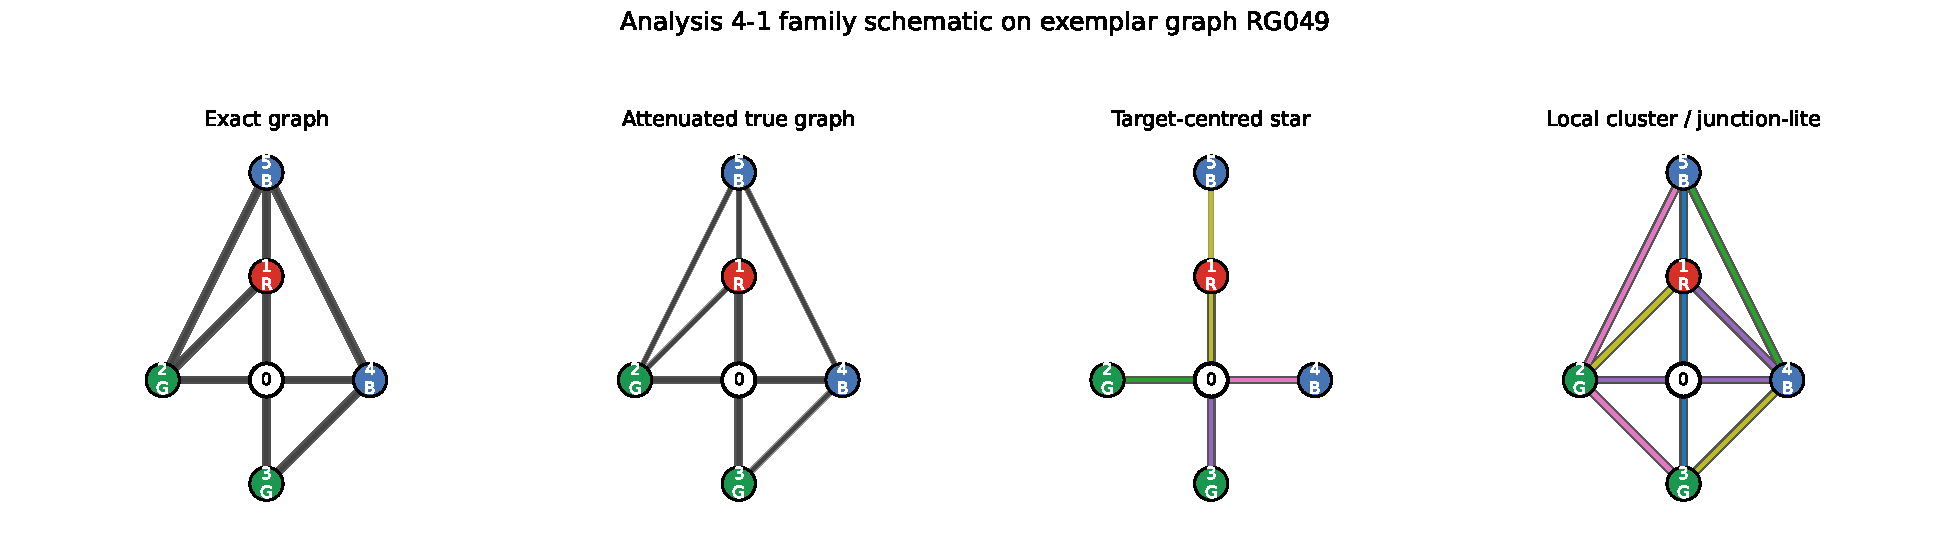
\includegraphics[width=\textwidth]{analysis-4-1_fig1_family_schematic.pdf}
\caption{Conceptual distinction between exact inference, attenuation on the true graph, a target-centred star rewrite, and a local cluster rewrite.}
\end{figure}

\section{Conclusions against the TODO}
\begin{enumerate}
    \item The family set stays within the required range and is simulation-ready.
    \item Structural rewrites are clearly separated from parameter variation.
    \item The pure local log-evidence heuristic should be absorbed into $M_0$ rather than treated as a separate family.
    \item The six-family set above is the recommended input to Analysis 4-2.
\end{enumerate}

\bibliographystyle{apalike}
\bibliography{../../manuscript/library}
\end{document}
